\chapter{Introduction}

\section{Background}
\subsection{Technology}

The technology section will be based on the new ICT based virtual coaching solution vCare. 

The basic concept of vCare is carried out by a central eHealth platform that serves central infrastructure services. The platform obtains the information delivered by sensors or gained by the direct interaction between the patient and the virtual coach. The devices added to this platform is a camera, microphones and Kinect which makes the platform able to track movements. The information from the devices are conducted by a real-time processor. Beside the platform the infrastructure delivers supporting services to improve the quality of life of patients. The service provides physical and cognitive exercises as well as education material within nutrition and life behaviour. This service will be extended with a care pathway and a knowledge layer that enables personalized exercises and material for the given patient. Based on algorithms the virtual coach is flexible regarding the patients’ needs and hereby able to make specific rehabilitation programs. The platform can be implemented on different devices, e.g., tablets, smartphones, TV screens etc. \cite{Technical}. 


\subsection{The Danish Healthcare System}

The establishment of the Danish Healthcare System started in the eighteenth century. The first hospital was placed in Copenhagen and it opened in 1757. This hospital is still functioning and is today known as Rigshospitalet. Outside the capital small hospitals were built during the late eighteenth century. Even then the hospital was partly financed by taxes, patient payment and charity. In the late nineteenth century every thirteenth Dane was a member in a sick-benefit association which the Danish Government co-funded. The Danish Welfare State has it's root in 1933 where the Social reform was founded. With this reform for Danes with a low income it became a demand that they were members of a sick-benefit association. During the thirties taxes gradually became the dominant finance source to the Danish Healthcare System.\\ 
The sick-benefit associations were shut down in 1973 and replaced by public health insurance. The Danish public health insurance is paid by the Danes themselves within taxes. But the insurance provides free care for everyone regardless of income and residence. This public health insurance includes hospital stays, surgery, visits to a GP and specialist'. Furthermore, it provides partly funding for dentist, physiotherapist, chiropractor, podiatrist and contributes to medicine.   \\

\subsubsection{The structure og the Danish Healthcare System}
Every healthcare system consists of users, healthcare institutions and the financial third part, besides the fundamental financial mechanism user fee, tax and budgets/rates. This is described with the tripartite model in \cref{Trepartmodel}. The A, B and C is the financial mechanism and 1, 2 and 3 is the consistence of the healthcare system. The model shows how a third part is pushed in between the users and the healthcare institutions. This third part creates equality between users as much as possible. The constellation of finances differs from country to country. Denmark is mostly funded by the Government through taxes whereas US citizen needs health insurance to pay the for these services \cite{sundhedsvaesen}. \\


\begin{figure}[H]
\centering
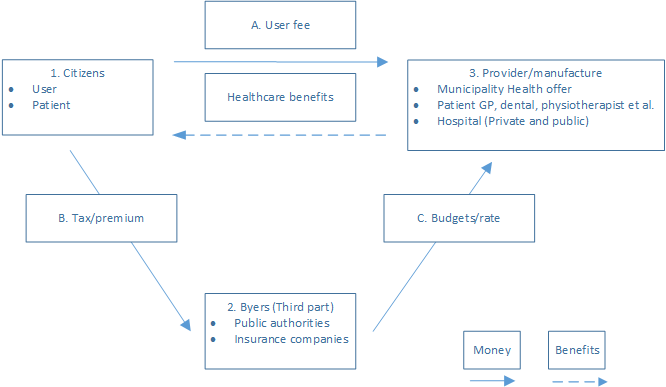
\includegraphics[width=1\textwidth]{Figure/thirdpart.png}
\caption{Tripartite model \cite{sundhedsvaesen}}
\label{Trepartmodel}
\end{figure} 

In 2007 the Danish State made big structural changes throughout the healthcare organisation. Municipalities were combined which meant a change from 275 municipalities to 98. The 14 counties were replaced by five regions. The Danish Healthcare System was thereby organized in three levels: State (National level), region (regional level) and municipalities (local level) \cite{indenrigs, Healthcareindk2}.\\
The municipalities have multiple tasks but in the health area they administrate general practitioners, home nursing, public healthcare, school health service, child dental treatment, prevention and rehabilitation\cite{sundhedsministeriet}. \\
The five regions are responsible for the secondary sector which is mainly the hospital sector. Each region is able to organize their services accordingly to their regional needs. They may adjust within the national legal limits, but the region will be responsible of procurement of staff and equipment.\\
The states task is to initiate, coordinate, and advise. Furthermore, the job is to establish goals for the national health policy\cite{sundhedsministeriet}. In Denmark a ministry takes care of this job. The ministry changes over time but in 2015 the name of the ministry became Ministry of health \cite{ministryofhealth}. This ministry is responsible for establishing the overall framework for the provision of health and elderly care.

The Ministry of Health is constantly seeking to improve the sector both in quality and efficiency at a minimum cost. Hereby the ministry set up some goals for the future and one of them is to minimize bed days. "As a result of the modernisation process, the number of bed days is expected to be reduced by 20 percent, and outpatient treatment to be expanded by 50 percent from 2007 to 2020" \cite{Healthcareindk2}. %jeg mangler en kilde på ovenstående minimum cost.


 %in 1927 there was a total of 160 somatic hospitals in Denmark.....nu er der kun ... og det gør at






\subsubsection{Finances}

The region is financed by four subsidies: Block grant from the state(75\%), state activity-related subsidy(5\%), local contribution(10\%) and local activity-related contribution(10\%). The block grant from the state is distributed with the consideration of differences inside the regions which will give the regions equal prospect of providing healthcare services. The rest of the subsidies are divided in three different types of distribution, this is partly to encourage the regions and municipalities to increase activity and efficiency \cite{sundhedsministeriet}.

The municipalities are financed with a block grant from the state but also council taxes which differs in municipalities. The regions receive activity-based subsidy from the municipality which means that the municipality pays the region money depending on the number of hospitalisations and treatments performed by the hospital of the municipalities citizens. Due to this constellation the municipality has incitement to reduce demands for hospitalization and other regional healthcare services \cite{Healthcareindk2}.
The finance structure in the Danish Health care system aims to strengthen health clinical production and responsiveness with free choice of hospital in combination with the activity-based financing. Throughout the structure plan in 2007 the municipalities where given a financial incentive to keep their citizens healthy \cite{DKhealthreview}.



\subsubsection{Preventive healthcare}

As a part of the local government reform in 2007 preventive healthcare became an important part of the Danish Healthcare System. The vision was to improve quality of life and impact the lifestyle related diseases like cancer and cardiovascular diseases which are the dominant cause of death today in Denmark. Furthermore, it included focus on risk factors as tobacco, alcohol and lack of exercise. The municipalities were given the primary responsibility for preventive health \cite{sundhedsministeriet}.

\subsubsection{Rehabilitation}

Rehabilitation, including physical and mental training, programmes are offered for all citizens by the municipalities. The training and the rehabilitation of a patient may be initiated at the hospital and carried on within the municipality when the patient is discharged. This means that the municipality will be responsible for the rehabilitation after discharge. Rehabilitation helps the patient to regain functional abilities and helps them to become self-sufficient. Some will receive rehabilitation free of charge whereas others may pay partly from their own pocket. This depends on the type illness \cite{Healthcareindk2, retningsrehab, WHO}.

%Her skal noget mere på....


\subsubsection{Digitization in the healthcare system}

Denmark is known for extensive digitization and electronic communication in the Healthcare Systems and the use of health data. Denmark made standards for electronic communication years ago and the result of this is an almost digitalized communication within the healthcare sector. Health records, laboratory test results and hospital referrals are all nearly collected as electronic data. 
Multiple ICT and digital workflow are completely integrated, this marks Denmark as a frontrunner in deployment of e-health.\\
Telemedicine is a big part of the digitalization plan in Denmark where five initiatives is to be the foundation of future telemedicine infrastructure in Denmark. "The goal is to have a digital infrastructure and IT architecture in place within the foreseeable future, so that relevant information can be exchanged across the healthcare system and other sectors" \cite{Healthcareindk2}.
In 2011 Denmark started a project for telemedicine throughout the country. The five regions jointed forces to make an strategy how to develop telemedicine in an wider scale and combine it with effective shared knowledge. For this to happen a board has been chosen and it is the National Board og E-Health \cite{DKhealthreview}. % Her skal komme noget om fælles udbud telemedicin 



%Skal vi have noget om data med?
%Noget med udbud på it systemer over en hvis pris?

%DE snakker om cardiovaskulær patient på side 41 hvor de nævner guidelines i forhold til rehabilitering - den skal vi finde i fuld skala, her en kort udgave: https://www.sst.dk/da/udgivelser/2015/~/media/E21E277725B8408698A96502F4BEF472.ashx
% Nedstående er mulige ting der kan anvendes forskellige steder i rapporten
 %"The patients' self-monitoring of the disease should be enhanced and technologies for self-monitoring should be evaluated and the quality of the monitoring should be assured."\cite{NationalBoardofHealth}
\subsubsection{Treatment of Cardiac patients}

In 2010 treatment packages for non-acute heart disease was introduced in Denmark. This package included a process consisting of investigation, diagnosis, treatment and rehabilitation. The Danish Health Authority decided to offer the package deal in 2010. With this alteration the patient will achieve a more simple and coherent treatment with better quality. 
The progress for the patient will be described in the next section. \\

Step 1 Preliminary assessment and referral: when a patient feels ill they contact their general practitioner (GP), unless it is acute. It is the GP's job to carry out preliminary examination and give the patient to the right kind of treatment if necessary. The GP should include the patient in choice of treatment plan and decide if the patient needs to be admitted to the hospital or an outpatient visit to the hospital.\\
Step 2 Investigation and treatment: the investigation and treatment of cardiovascular patients differs from diagnosis to diagnosis. Common is that the knowledge of comorbidity is important due to stabilization and treatment of the concurrent disease throughout the treatment of the cardiovascular disease. The health facility will form a treatment plan in corporation with the patient. \\
Step 3 Planning follow-up on treatment, rehabilitation and palliation: At the end of treatment the cardiology department/specialist practice performs a systematic assessment of needs. The needs assessment is carried out in collaboration with the patient and perhaps relatives. 
Step 4 Follow-up: When the patient has been discharged from the hospital the treatment will pursue in the outpatient visit while others will pursue follow-up at their GP's. \\
Step 5 Rehabilitation and palliation: patients with heart disease should systematically perform a need assessment in order to offer rehabilitation and palliative action based on patient needs and heart disease. Rehabilitation with heart patients is mainly performed with focus on disease coping, nutrition, physical training, tobacco cessation and work retention. Furthermore, it aims to improve the individuals physical and mental state of health. The rehabilitation is primarily placed in the municipalities. The effort of rehabilitation planning should origin in the patients functioning, preferences and resources. Motivation, participation and adherence of achieved change of behaviour are important elements in the rehabilitation process. After heart disease the patient is at great risk of developing anxiety and depression and it is therefore important that physicians related to the rehabilitation process are observant. 
Patients with heart disease experience varying periods of worsening of the disease along with more calm periods. In connection with impairments and possible subsequent hospitalization, there will often be uncertainty as to whether the patient survives. This is always a burden for both the patient and the relatives. In this regard, it is important for health professionals to pay attention to and assess the patient's and their dependents' palliative needs and problems associated with heart disease, and that the need is assessed on a regular basis to prevent efforts from initiating too late \cite{behandlingsforlob}.

%Nedstående skal indsættes et sted

The number of hospital has declined throughout the past 28 years. This concerns both Acute, long-term and psychiatric care sectors. Through changes in treatment options the average length of hospital admission have declined as well. The average lenght of the admission has decreased with 40\%, which makes Denmark the country with the shortest length of stay in Scandinavia. the decline is due to more effective treatments and out patient treatments  \cite{DKhealthreview}


\subsection{Target Group and Market Segment}

By introducing telemedicine the rehabilitation process is brought directly to patients' homes and mostly targets people with chronic conditions, which includes cardiac patients. Telemedicine rehabilitation is used to prevent hospitalization, to improve patients' feeling of safety, to empower patients to manage their own chronic condition and hereby improve patients' quality of life \cite{Emergence}. 

The need for cardiac rehabilitation is evaluated for all patients with heart disease. This includes both patients who have had a balloon dilation or by-pass surgery and patients with stable ischemic heart disease.
Patients with heart failure, pacemaker or patients who have had heart-valve surgery or cardiac transplantation are also being evaluated for the purpose of cardiac rehabilitation \cite{Rehabilitering}. By this statement it is seen, that this invention will involve a large target group.

To teach cardiac patients about their illness and how they are able to influence the course of the disease, results in a reduced risk of dying. Furthermore, research shows that rehabilitation programs with physical exercise reduce cardiac mortality \cite{Hjerteforening}.    


\section{Problem Statement}
More than half of the danish citizens over the age of 55 suffer from a cardiovascular disease. Furthermore, cardiovascular diseases are one of the most common causes to death in Denmark. The total cost of treating cardiovascular patients at the Danish Healthcare System was 5.5 billion DKK in 2015. Every year approximately 55.700 Danes is diagnosed with cardiovascular disease.   

Nearly 107.100 Danes are hospitalized every year for cardiovascular disease and almost 73.100 Danes are yearly at one or more consultations at the hospital. Approximately 23 percent of the cardiovascular patients are readmitted into the hospital within 30 days after being discharged. It has been proven, that cardiac rehabilitation results in a reduction in deaths caused by cardiovascular diseases and the need for readmissions \cite{Hjerteforening}.

All this indicates that cardiovascular patients constitute a large part of the Danish states economy. This leads to our problem statement which is:

\begin{itemize}
	\item What impact would an ICT solution for rehabilitation have on both cardiovascular patients and the Danish Healthcare System?
	\item How can ICT be used to shorten hospital stay for cardiovascular patients?
	\item Which barriers/challenges can such system meet in implementation?
\end{itemize}

\subsection{Delimitation}
This project is limited only to be focusing on healthcare in Denmark and how the technology within rehabilitation will have an essential impact on the Danish Healthcare System. However, the project will be compared to related ICT solutions in EU as scientific articles based on The Danish Healthcare System is limited in this research area. 

Relevant data on how the Danish Healthcare System is establish will mainly be based on literature found in books and on websides were guidelines, statistics and the historical development is being published. 


